\documentclass[journal,onecolumn,10pt]{IEEEtran}
\usepackage{amsmath,graphicx,url}
\renewcommand{\thetable}{S\arabic{table}}
\renewcommand{\thefigure}{S\arabic{figure}}
\begin{document}
\title{Supplementary Analyses: Cellular Throughput Recalibration}
\author{Md. Moazzem Hossain Majumder}
\maketitle
\begin{abstract}Supporting analyses preserve the original experimental protocols, results and limitations. The main article presents the narrower acquisition-cost and selective-risk argument. These retrospective analyses are not independent confirmatory trials.\end{abstract}
\begin{IEEEkeywords}
Cellular throughput, conformal prediction, measurement methodology, missing radio telemetry.
\end{IEEEkeywords}

\section{Question and related work}
An application that chooses a sending rate before a download needs to know how often its forecast exceeds delivered throughput and how much usable rate it gives up to reduce those violations. We ask how those quantities change when an operator has only a few labeled examples from the destination network. The contribution is an empirical comparison on released traces, with a common predictor and a fixed test suffix across label budgets. Prior work characterizes the underlying campaigns \cite{kousias2024data,caso2024}, additive prediction with missing observations \cite{jacobson2025}, and conditional calibration under missing covariates \cite{zaffran2023}. The BAMMO-inspired baseline uses our pattern-specific boosted trees. We did not replicate the original authors' implementation. Grouping by recorded telemetry availability gives a simple comparator. Its interpretation depends on support within each group.

Our central question is how constrained, delayed and unsuccessful calibration feedback changes selective cellular throughput commitments under chronological distribution changes. The clock replay supplies the primary evidence. On the later source operator the ten-label tree violated 67 of its 122 measurable positive commitments. On the destination operator it violated two of only three. The following questions guide the analysis. Does measured risk resolve the target across all issued commitments? Does the session-trained tree retain its operating point on a fixed clock? Do more recent or telemetry-specific calibration labels improve the risk and supported-rate tradeoff on the same forecast opportunities? We answer these questions with a decision ledger, matched predictors and chronological prefix comparisons. The external analyses distinguish transfer of a fitted predictor from transfer of its calibration offset.
Narayanan et al.\ mapped and predicted commercial millimeter-wave throughput \cite{narayanan2020}, while Kousias et al.\ modeled performance in non-standalone networks \cite{kousias2024model}. Our benchmark evaluates how much measured rate remains supportable when an existing point forecast receives only a short destination calibration prefix.
The study makes three empirical contributions: an auditable acquisition-and-decision ledger separating initial labels, new attempts, failures and effective updates; a full-suffix comparison that distinguishes equal caps from equal realized query cost; and an offer-level decomposition explaining cohort-specific service--risk trade-offs. We ask how failed and delayed feedback affects the implemented decisions, how acquisition constraints change reliability and supported throughput, whether realized-cost matching changes conclusions, and when increased service sacrifices reliability. Fixed archive delays are modeled rather than experimentally randomized, so we do not isolate their causal effect.

Selective prediction already connects acceptance frequency and conditional risk \cite{geifman2017}, adaptive conformal inference updates a nominal level online \cite{gibbs2021}, and conformal risk control calibrates monotone losses under explicit assumptions \cite{angelopoulos2024risk}. Costly-label stopping and semi-bandit feedback have also been studied \cite{ilyas2026,ge2025}. Our empirical accounting framework evaluates these mechanisms under real cellular traces.

\section{Decision criteria and contribution}
The primary contribution is a reproducible empirical test of whether a reliability conclusion survives explicit accounting for positive offers, unobserved outcomes and independent collection units. The algebra below makes the decision rule auditable. Selective prediction already relates conditional risk to acceptance frequency; our study applies that relationship to minimum-rate promises with incomplete outcomes and measured service.

Let $N$ denote eligible issued forecasts (including zero commitments), $M$ the positive promises, $e$ observed violations, and $m$ positive promises without an outcome. For a completed ledger let $R$ be failure across all issued promises, $R_+$ failure conditional on a positive promise, and $A=M/N$. Since a zero promise cannot violate a nonnegative rate, $R=A R_+$. Thus a ceiling $R\leq\alpha$ permits conditional failure as high as $\min(1,\alpha/A)$. The earlier selection experiment illustrates why an overall risk ceiling can coexist with poor positive-promise reliability.

When outcomes are unavailable, the sharp bounds are
\[
 R\in[e/N,(e+m)/N],\qquad
 R_+\in[e/M,(e+m)/M]\quad(M>0).
\]
Each endpoint is attained by assigning every unobserved positive promise an outcome equal to its promise or zero, respectively. These bounds require a well-defined nonnegative latent rate at each opportunity. They do not identify service after logging ends. For a chosen positive-promise tolerance $\alpha$, the recorded ledger meets the tolerance under every completion exactly when $e+m\leq\alpha M$; it fails under every completion when $e>\alpha M$. Otherwise the missing outcomes leave the decision unresolved. A policy with $M=0$ has undefined conditional risk and no positive service. Report $A$ and measured supported throughput alongside this decision. The latter conditions on observed outcomes and cannot identify throughput on unrecorded service attempts.

This finite-record test does not constitute a new distribution-free population guarantee. It connects the issued ledger to an operationally interpretable criterion and supplies a falsifiable test for the empirical claims. The main evidence is the clock replay and independent archives. Session-defined endpoints, alternative models and budget frontiers provide sensitivity analyses.
\subsection{Budgeted commitment and recalibration}
We investigate whether an explicit budget for new calibration queries changes the preferred commitment policy. Prior cellular work already studies global, grouped and adaptive rate bounds \cite{sirhan2026}; missing-value conformal prediction treats input patterns \cite{zaffran2023}; recent methods address costly labels and semi-bandit feedback \cite{ilyas2026,ge2025}. These precedents prevent a novelty claim for their generic combination. Our contribution is the causal acquisition ledger, the unresolved-response residual bound and a matched test of their consequences in the released cellular traces. MARUR is a provisional controller used to test that design.

Let $Q_t$ indicate a new calibration query chosen at issue time $t$, $C$ the new-query cap, and $L_t\geq0$ the committed rate. The empirical design objective is to maximize supported measured throughput subject to $\sum_t Q_t\leq C$, a positive-offer requirement, and an acceptable upper conditional failure fraction $(e+m)/M$. The ten initial labels are pre-test successes; their original failed acquisition attempts are unknown. Lag-rate feedback needed for forecasting remains outside the charged query budget. These constraints define an evaluation aspiration, not an optimization solved by the controller. It neither optimizes utility nor enforces positive-offer frequency or conditional risk. We retain the legacy hybrid index $B=10+C$ only to identify archived runs; it is not total measurement cost.

At a tick with an available prior rate, the controller computes $L_t=\max(0,p_t-q_t)$. Its ten-entry residual window contains initial successful labels and completed query scores. At a nominal level of 0.1, a nine- or ten-entry finite-sample quantile is the maximum residual. If a requested outcome is unobserved, $p_t-y_t\leq p_t$ for nonnegative $y_t$, so we insert $p_t$ as a conservative residual bound. MARUR uses a pattern-specific 90 percent quantile when at least nine entries share the current LTE/NR availability pattern, otherwise the pooled quantile. Fewer than three entries in the current pattern triggers abstention. It requests a new outcome when the pattern differs from the most recent response or that response is at least sixty minutes old. A failed response resets the age and pattern trigger even when the drop-missing variant discards its score. There is at most one outstanding request, and each request is charged before reading its outcome. Budget exhaustion prevents new requests; an outstanding paid response can still update the window. Simultaneous forecasts share the same state.

Frozen calibration, queries every fifteenth eligible tick, and immediate queries whenever possible provide baselines. A delayed, budgeted ACI comparator updates its nominal error level by $a\leftarrow a+0.05(0.1-\mathrm{error})$ on requested feedback. Unresolved queried positive offers count conservatively in this update; rates are capped at the point forecast for every nominal level. These changes and partial feedback prevent inheriting full-feedback ACI guarantees. Ablations remove pattern-dependent decisions, discard unresolved responses while still charging them, or use periodic acquisition. We report every new-query cap $C\in\{0,10,40\}$, both predictors, and a simulated condition that hides feedback from every fifth eligible opportunity from the controller while retaining the recorded label for evaluation. All thresholds were specified for this experiment after earlier archive analyses; the experiment is exploratory.

\subsection{Executable decision sequence}
The implementation initializes a ten-score FIFO buffer, a completed-response timestamp/pattern, eligible ordinal, pending request and query counter. At each distinct issue time it first receives requests whose horizons have closed. An observed response inserts $p-y$; an unsuccessful response inserts $p$, except in the drop-missing ablation. Every completion updates cooldown and pattern even if its score is discarded. It then processes simultaneous rows in ID order using the same buffer: compute the pooled or supported-pattern quantile, apply nonnegativity and the pattern gate, and record the commitment. A new request is charged only if the policy trigger fires, the new-query cap is unspent and none is pending. The stored commitment is used when an ACI response updates its nominal level. A final outstanding response is recorded even if no later forecast can use it. This sequence distinguishes completed feedback from observed evidence and admits no future outcome before its horizon closes.

For $T$ rows and window size $W$, sorting and per-row score ordering require $O(T\log T+TW\log W)$ time. Controller state is $O(W)$, but the full pandas replay retains inputs and action/response ledgers, requiring $O(T+Q+W)$ memory for $Q$ new requests. The full policy-specific pseudocode and state semantics are supplied in the implementation specification.

\section{Measurements and prediction time}
The earlier campaign uses the active throughput CSV in Zenodo 8224890. We take the last available mean download throughput at a DQA completion marker within a campaign and convert kb/s to Mbps. In the later active archive (Zenodo 14073311), we use 43 Ookla traces and process each operator's nonnegative numeric mean-download series separately, converting its documented column units to Mbps. With reset segmentation the releases yield 1,132 operational sessions and 1,001 eligible forecast pairs across development and evaluation. The main evaluation uses only held-out suffixes.
Each forecast uses the preceding result, elapsed time since that segment ended, its duration, recent radio measurements and availability indicators, and scenario. Among the 1,001 eligible pairs, 585 have only LTE measurements and 416 have both LTE and NR. No eligible pair lacks LTE. Consequently, grouping by NR presence and grouping by the two radio indicators define the same partition in this sample. In the later archive, the first throughput reading triggering a reset identifies the prediction time retrospectively. An online deployment would need an independent test-start signal. Even when predictors exclude that reading, selecting forecast times from the outcome trajectory can change the evaluated population. The primary protocol allows up to 60 seconds of lag age. Missing indicators describe what the logger observed. A missing NR signal by itself cannot identify a particular network state or its cause. Lagged throughput requires feedback from completed tests throughout evaluation. A budget of zero refers only to target labels used to fit the calibration offset.

E0 uses five successive blocks of earlier Op1 collection days for training, validation, source calibration, target prefixes and testing. The first three blocks contribute 57, 9 and 33 observations. The benchmark freezes that predictor and source offset for all four regimes. E1 moves to later Op1, E2 to earlier Op2 and E3 to later Op2. Transfer calibration and test blocks use the first approximately 40 percent and last approximately 60 percent of target days, respectively, with integer day boundaries. We take the first $K$ eligible sessions in timestamp order from the calibration pool. E0 has ten available, so its fifteen-session comparison is unavailable. Cross-operator analysis on contemporaneous campaigns is retrospective.

\section{Calibration and metrics}
Let $f$ denote the frozen histogram gradient boosting model and $y$ the endpoint throughput. Split calibration orders the signed scores $f(x_i)-y_i$. For $n$ finite scores, take rank $r=\lceil(n+1)(1-\alpha)\rceil$ in ascending order. When $r>n$ we use positive infinity. The lower forecast is $L=\max(0,f(x)-q)$. A tie at the bound counts as covered. Since $r\le n$ is equivalent to $(n+1)(1-\alpha)\le n$, finite scores yield a finite selected order statistic exactly when $n\geq\lceil1/\alpha\rceil-1$. At $\alpha=0.10$ the first finite rank occurs at nine scores and selects their maximum. Ten also selects the maximum. This calculation gives no estimate of the campaign size needed for a useful rate.
The rank argument follows the standard conformal construction \cite{vovk2005algorithmic}. Under exchangeability of calibration and future scores conditional on an independently fitted predictor, the rank construction yields marginal coverage of at least $1-\alpha$. The data do not establish this assumption across consecutive sessions, dates or networks. With an infinite target quantile the benchmark uses a frozen source offset. Its target-domain coverage is empirical. The grouped rules try a finite group offset, then a finite pooled target offset, then the source offset. The row gate is three and the session gate one. A group still needs enough scores for a finite rank. The RAT proxy groups by recorded NR presence. The missingness rule also uses LTE availability.

We compute $V=\sum_i\mathbf{1}\{y_i<L_i\}/N$ and $U=\sum_i\min(L_i,y_i)/\sum_i y_i$. A near-zero bound can yield few violations while providing little usable throughput. In this complete-outcome session analysis $N$ is the scored count. For the clock and MARUR ledgers we separately retain eligible-issued and measured counts, and compute $U$ only over observed eligible outcomes. These are offline measures. The benchmark does not measure an application outage, a contractual breach or a revenue loss.
\begin{table*}[!ht]
\centering\small
\caption{Source validation errors in Mbps and measured fit time in seconds.}
\begin{tabular}{lrrr}
\hline
Model & MAE & RMSE & Seconds \\
Persistence & 3.22 & 7.21 & 0.000 \\
Ridge & 6.03 & 8.78 & 0.041 \\
HistGradientBoosting & 11.00 & 12.00 & 1.550 \\
BAMMO & 15.46 & 23.86 & 0.383 \\
QuantileGBM p10 & 5.01 & 8.68 & 0.073 \\
GPU ThroughputResNet & 5.85 & 8.33 & 0.745 \\
\hline
\end{tabular}
\end{table*}

\begin{table*}[!ht]
\centering\small
\caption{Test sessions and lower-bound performance by regime and target prefix. P denotes point, G global, R radio access and M missingness groups. V denotes violations and U supported fraction.}
\begin{tabular}{lrrrrrrrrr}
\hline
Regime/K & N & PV & PU & GV & GU & RV & RU & MV & MU \\
E0K0 & 41 & 0.4390 & 0.3705 & 0.1220 & 0.1761 & 0.1220 & 0.1761 & 0.1220 & 0.1761 \\
E0K1 & 41 & 0.4390 & 0.3705 & 0.1220 & 0.1761 & 0.1220 & 0.1761 & 0.1220 & 0.1761 \\
E0K2 & 41 & 0.4390 & 0.3705 & 0.1220 & 0.1761 & 0.1220 & 0.1761 & 0.1220 & 0.1761 \\
E0K5 & 41 & 0.4390 & 0.3705 & 0.1220 & 0.1761 & 0.1220 & 0.1761 & 0.1220 & 0.1761 \\
E0K8 & 41 & 0.4390 & 0.3705 & 0.1220 & 0.1761 & 0.1220 & 0.1761 & 0.1220 & 0.1761 \\
E0K9 & 41 & 0.4390 & 0.3705 & 0.0976 & 0.0858 & 0.0976 & 0.0858 & 0.0976 & 0.0858 \\
E0K10 & 41 & 0.4390 & 0.3705 & 0.0000 & 0.0285 & 0.0000 & 0.0285 & 0.0000 & 0.0285 \\
E1K0 & 139 & 0.4101 & 0.4102 & 0.1655 & 0.1717 & 0.1655 & 0.1717 & 0.1655 & 0.1717 \\
E1K1 & 139 & 0.4101 & 0.4102 & 0.1655 & 0.1717 & 0.1655 & 0.1717 & 0.1655 & 0.1717 \\
E1K2 & 139 & 0.4101 & 0.4102 & 0.1655 & 0.1717 & 0.1655 & 0.1717 & 0.1655 & 0.1717 \\
E1K5 & 139 & 0.4101 & 0.4102 & 0.1655 & 0.1717 & 0.1655 & 0.1717 & 0.1655 & 0.1717 \\
E1K8 & 139 & 0.4101 & 0.4102 & 0.1655 & 0.1717 & 0.1655 & 0.1717 & 0.1655 & 0.1717 \\
E1K9 & 139 & 0.4101 & 0.4102 & 0.0719 & 0.0725 & 0.0719 & 0.0725 & 0.0719 & 0.0725 \\
E1K10 & 139 & 0.4101 & 0.4102 & 0.0719 & 0.0725 & 0.0719 & 0.0725 & 0.0719 & 0.0725 \\
E1K15 & 139 & 0.4101 & 0.4102 & 0.0719 & 0.0725 & 0.1007 & 0.0833 & 0.1007 & 0.0833 \\
E2K0 & 256 & 0.6211 & 0.4232 & 0.1641 & 0.1888 & 0.1641 & 0.1888 & 0.1641 & 0.1888 \\
E2K1 & 256 & 0.6211 & 0.4232 & 0.1641 & 0.1888 & 0.1641 & 0.1888 & 0.1641 & 0.1888 \\
E2K2 & 256 & 0.6211 & 0.4232 & 0.1641 & 0.1888 & 0.1641 & 0.1888 & 0.1641 & 0.1888 \\
E2K5 & 256 & 0.6211 & 0.4232 & 0.1641 & 0.1888 & 0.1641 & 0.1888 & 0.1641 & 0.1888 \\
E2K8 & 256 & 0.6211 & 0.4232 & 0.1641 & 0.1888 & 0.1641 & 0.1888 & 0.1641 & 0.1888 \\
E2K9 & 256 & 0.6211 & 0.4232 & 0.0234 & 0.0177 & 0.0234 & 0.0177 & 0.0234 & 0.0177 \\
E2K10 & 256 & 0.6211 & 0.4232 & 0.0234 & 0.0177 & 0.0234 & 0.0177 & 0.0234 & 0.0177 \\
E2K15 & 256 & 0.6211 & 0.4232 & 0.0234 & 0.0177 & 0.0977 & 0.0993 & 0.0977 & 0.0993 \\
E3K0 & 103 & 0.3301 & 0.3527 & 0.1262 & 0.1451 & 0.1262 & 0.1451 & 0.1262 & 0.1451 \\
E3K1 & 103 & 0.3301 & 0.3527 & 0.1262 & 0.1451 & 0.1262 & 0.1451 & 0.1262 & 0.1451 \\
E3K2 & 103 & 0.3301 & 0.3527 & 0.1262 & 0.1451 & 0.1262 & 0.1451 & 0.1262 & 0.1451 \\
E3K5 & 103 & 0.3301 & 0.3527 & 0.1262 & 0.1451 & 0.1262 & 0.1451 & 0.1262 & 0.1451 \\
E3K8 & 103 & 0.3301 & 0.3527 & 0.1262 & 0.1451 & 0.1262 & 0.1451 & 0.1262 & 0.1451 \\
E3K9 & 103 & 0.3301 & 0.3527 & 0.0291 & 0.0578 & 0.0291 & 0.0578 & 0.0291 & 0.0578 \\
E3K10 & 103 & 0.3301 & 0.3527 & 0.0000 & 0.0060 & 0.0000 & 0.0060 & 0.0000 & 0.0060 \\
E3K15 & 103 & 0.3301 & 0.3527 & 0.0000 & 0.0060 & 0.0000 & 0.0060 & 0.0000 & 0.0060 \\
\hline
\end{tabular}
\end{table*}


\section{Session-endpoint comparison}
Table~S1 reports source model selection. Table~S2 and Fig.~S1 show the full budget curve. Fig.~S2 compares observed subgroups. Persistence had a lower validation MAE than the histogram model on nine source-validation observations. We use the common histogram predictor to isolate differences between calibration rules. We examine persistence separately on the external benchmark and in the joint-shift analysis below. The point baseline exceeds the measured throughput in roughly one third to three fifths of held-out sessions. With source calibration, every regime exceeds ten percent violations at each tested budget below nine. At ten labels the global method records zero violations in E0 and E3, approximately seven percent in E1 and two percent in E2. In E3 it supports less than one percent of measured rate. At fifteen labels the grouped E1 rule exceeds the nominal target (0.1007), while grouped E2 increases supported fraction to 0.0993 with a violation rate of 0.0977. All four regimes give identical global and missingness-group results at ten labels when the pooled fallback is applied consistently. Thus this comparison provides no evidence of a grouping advantage at that budget. At ten labels the tree offsets were 27.81, 22.79, 28.70 and 30.29 Mbps, respectively. Clipping then produced zero rates on 65.85, 59.71, 75.00 and 93.20 percent of the suffixes. Group-level support existed for 54 of 539 forecasts; the remaining 485 used the pooled target. The identical bounds therefore reflect both fallback and coincident offsets.
\begin{figure}[!ht]\centering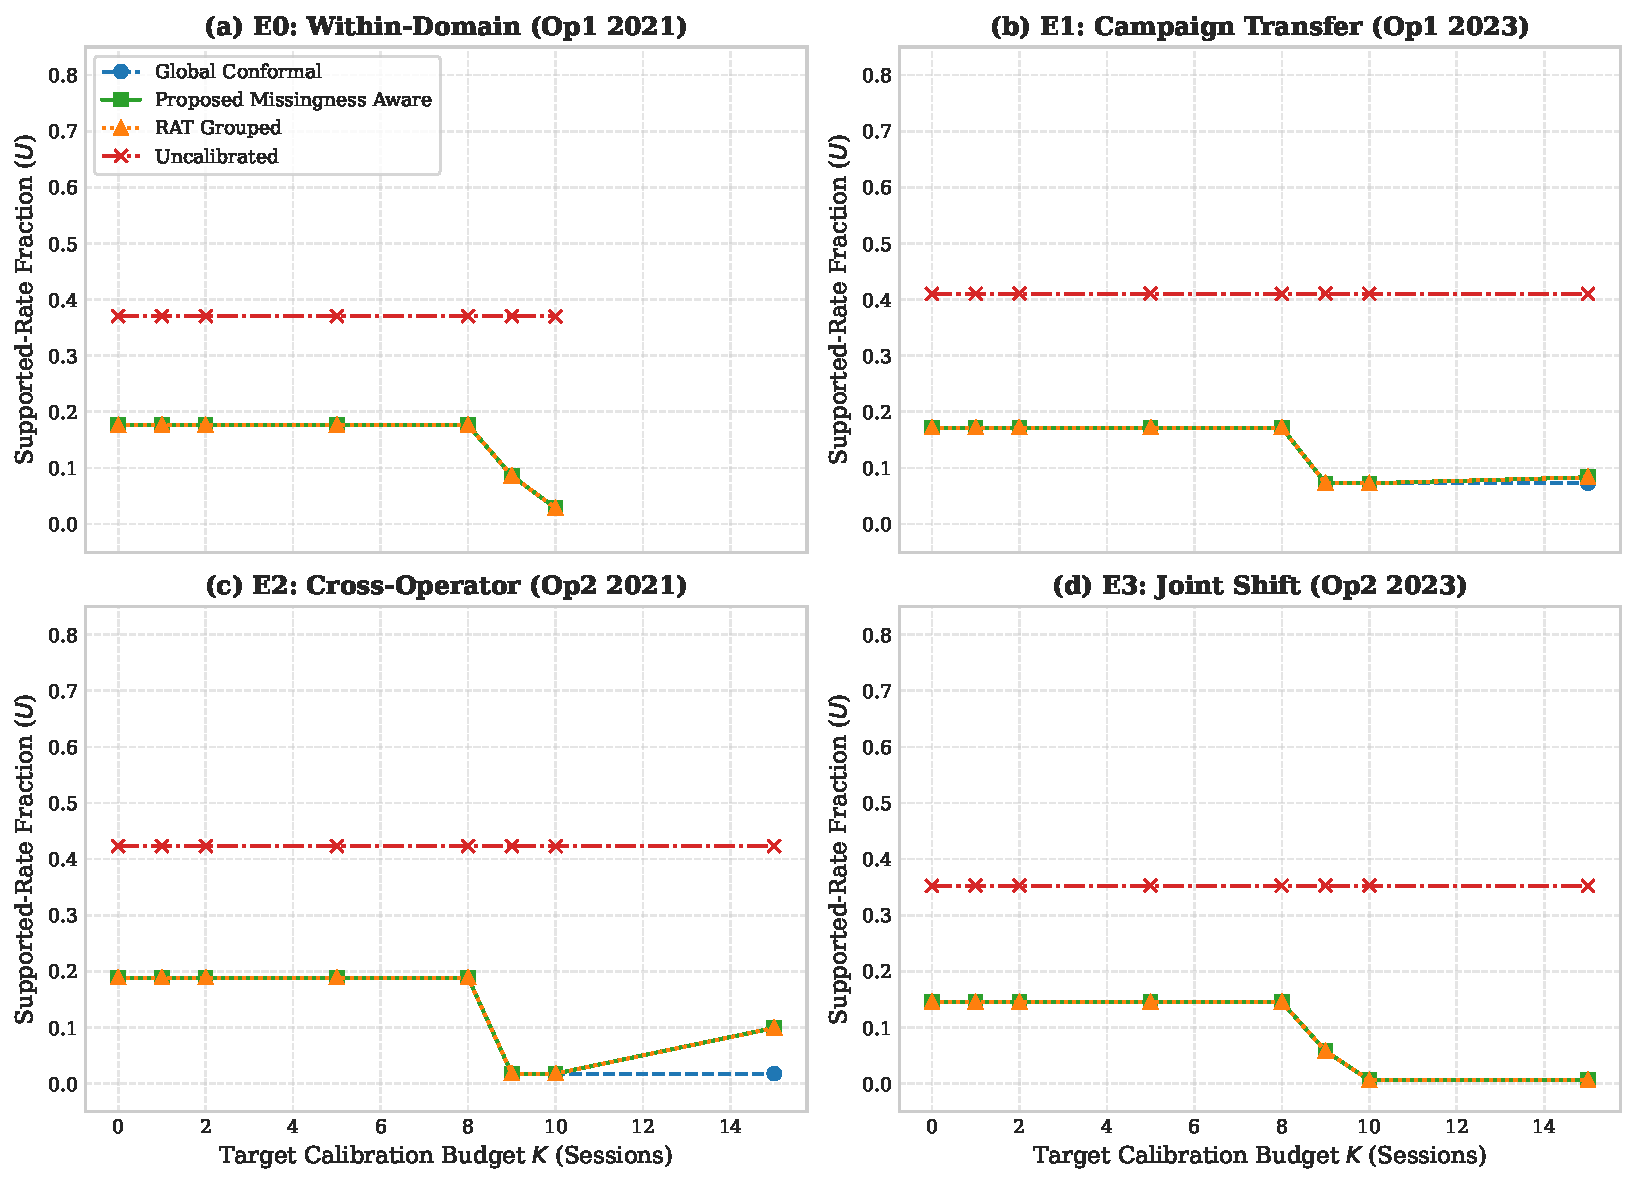
\includegraphics[width=.80\linewidth]{figures/fig1_budget_vs_usefulness.pdf}\caption{Performance across chronological calibration budgets. The same suffix is used at every available budget within a regime.}\end{figure}
\begin{figure}[!ht]\centering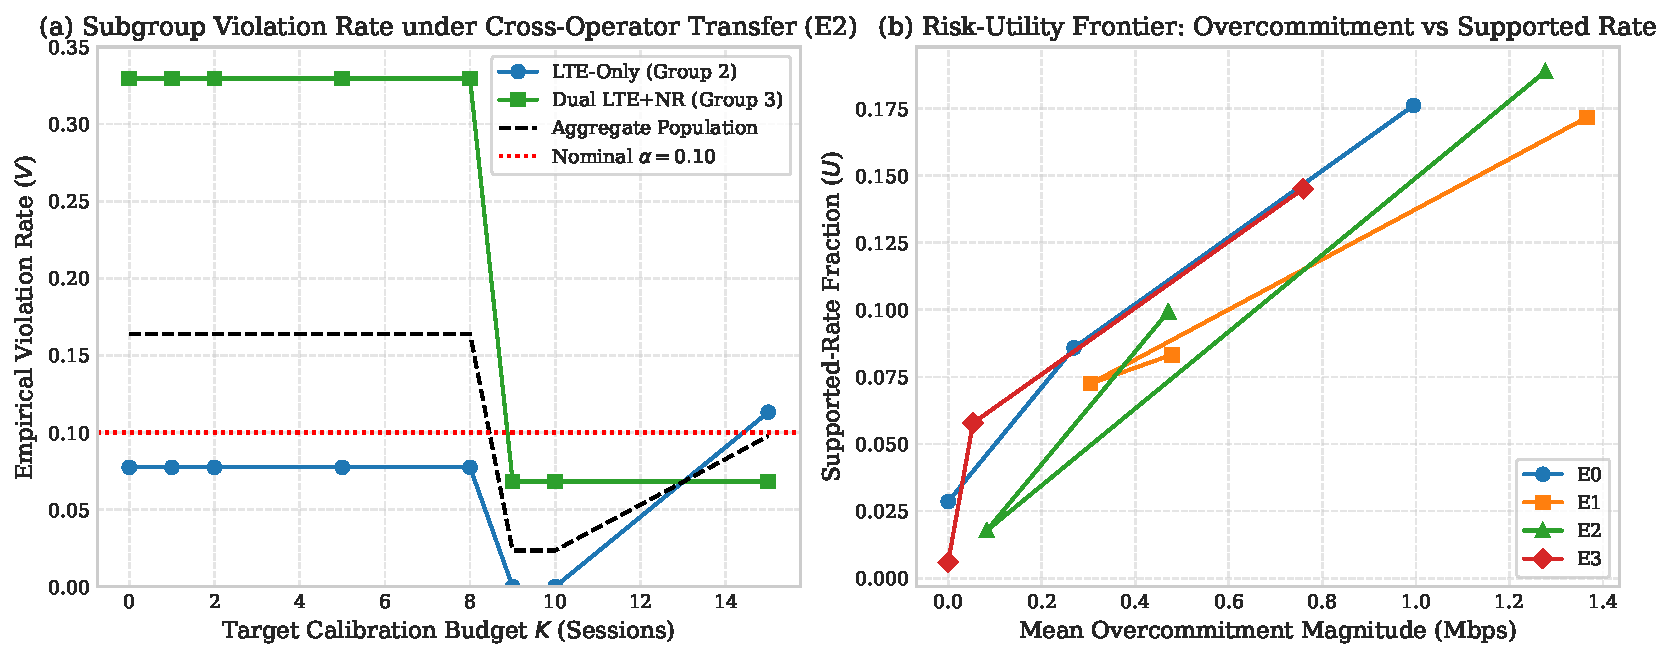
\includegraphics[width=.80\linewidth]{figures/fig2_subgroup_and_tradeoff.pdf}\caption{Subgroup performance and the empirical rate trade-off on the observed campaigns.}\end{figure}

\section{Sensitivity to the observational unit}
Table~S3 compares the operational units. After numeric filtering, reset starts a segment on a drop exceeding 5 Mbps to below 5 Mbps. Relative drop starts on a drop exceeding 2 Mbps to below 1 Mbps. The active-start rule begins on an upward crossing above 1 Mbps or a gap over ten seconds. All three retain the last numeric row as the target. The active-start rule therefore frequently attaches the subsequent idle tail to the preceding burst. Its endpoint can differ even on a continuously logged trace. We use it as an alternative-endpoint stress test. There is no independent truth label for a physical download boundary. The reset rule aligns with a reinitializing mean-rate series and preserves the original benchmark definition. Its agreement with actual test starts remains unknown. The sensitivity analysis evaluates all eligible later pairs with a source-fitted model. Its denominator differs from the held-out benchmark. After excluding zero endpoints from scoring while keeping the fitted predictor, burst violations remain 0.3742 and 0.4651 on the two operators. Thus zero endpoints explain only part of the shift. Relative drop also changes the sample and the rates. None of these heuristics establishes ground-truth session boundaries.
\begin{table*}[!ht]
\centering\small
\caption{Source-only sensitivity across all eligible later-campaign pairs.}
\begin{tabular}{lrrrr}
\hline
Boundary & Segments & Zeros & E1V & E3V \\
Reset & 584 & 23 & 0.1479 & 0.2523 \\
Drop & 712 & 23 & 0.1339 & 0.2172 \\
Burst & 930 & 183 & 0.4024 & 0.4918 \\
\hline
\end{tabular}
\end{table*}

Median durations were 76, 72 and 53 seconds for reset, relative drop and active start. On later Op2 the corresponding tree errors were 27.41, 22.67 and 14.99 Mbps, while supported fractions were 0.2559, 0.2360 and 0.1490. A smaller absolute error coexisted with more violations as the endpoint population moved towards small values.

\section{Uncertainty and secondary experiments}
Table~S4 reports the paired contrasts. We resample collection dates with replacement, retaining all sessions from each selected date and pairing methods within each draw. The percentile endpoints from 2,000 draws describe empirical between-date variability conditional on this fitted model and prefix. Two to eight observed dates per regime offer little information about the population of future dates. A zero contrast interval follows algebraically when bounds coincide. Shared routes, equipment and measurement schedules can induce dependence across dates.
\begin{table*}[!ht]
\centering\small
\caption{Grouped minus global at ten sessions. Exploratory paired date bootstrap percentile endpoints.}
\begin{tabular}{lrrrrrrr}
\hline
Contrast & Days & dV & Vlo & Vhi & dU & Ulo & Uhi \\
E0D & 2 & 0.0000 & 0.0000 & 0.0000 & 0.0000 & 0.0000 & 0.0000 \\
E1D & 7 & 0.0000 & 0.0000 & 0.0000 & 0.0000 & 0.0000 & 0.0000 \\
E2D & 8 & 0.0000 & 0.0000 & 0.0000 & 0.0000 & 0.0000 & 0.0000 \\
E3D & 7 & 0.0000 & 0.0000 & 0.0000 & 0.0000 & 0.0000 & 0.0000 \\
\hline
\end{tabular}
\end{table*}

The repository includes every date's estimates and leave-one-date-out contrasts. Single-prefix testing leaves calibration-prefix variability unmeasured. Thirty-, sixty- and 120-second sensitivity runs change the eligible cohort and covariates together. Sixty seconds is the selected primary window. The supplementary analyses also examine group-support gates and artificial removal of observed NR fields. Artificial removal tests model response to controlled masking and does not identify why telemetry was absent in the field.

Table~S5 and Figs.~S3--S5 report the feedback, weighting and decision analyses. The online experiment updates an offset after each observed label with a fixed step size. Its feedback requirements differ from static prefix calibration. This score-offset update is inspired by adaptive conformal inference \cite{gibbs2021}. The weighted experiment estimates source-to-target density ratios with a domain classifier and compares two clipping ranges. One variant uses calibration-pool covariates and the other uses unlabeled test covariates. The tight weight range is 0.1 to 10 and the wide range 0.01 to 100. Covariate-shift theory requires a stable conditional outcome law and appropriate density ratios \cite{tibshirani2019}. Estimated, clipped weights and small effective sample sizes limit this interpretation. The alpha sweep and convex offline cost proxy show how the chosen threshold or penalty affects the displayed trade-off. The secondary sensitivity fits can use regime-specific source splits and should be compared within their own protocols.
\begin{figure}[!ht]\centering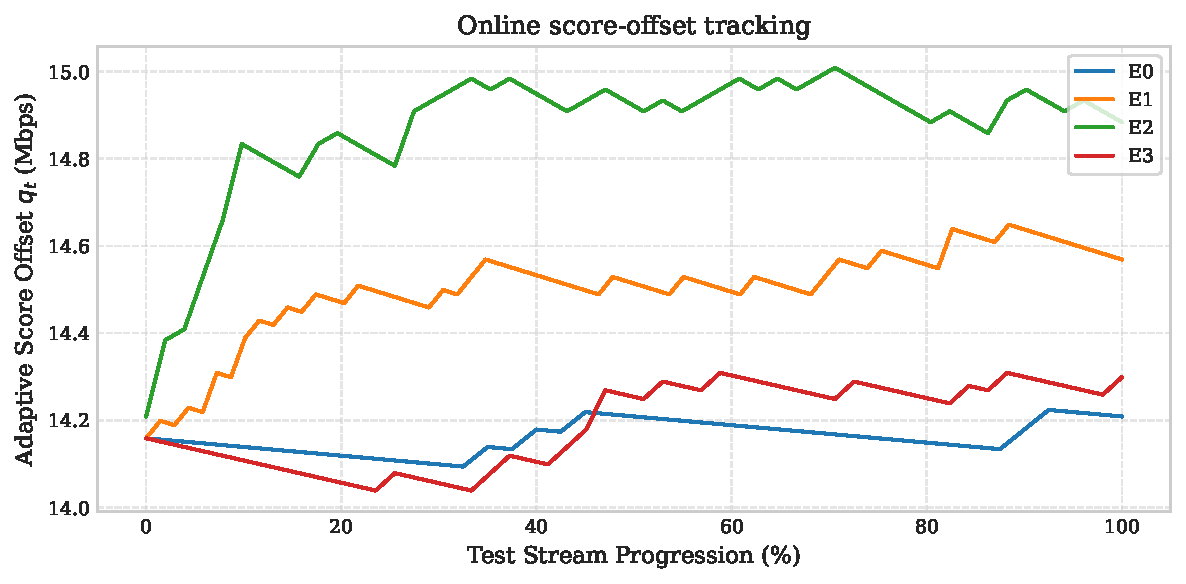
\includegraphics[width=.67\linewidth]{figures/fig3_aci_adaptation.pdf}\caption{Offset trajectory as labeled test sessions arrive in the online experiment.}\end{figure}
\begin{figure}[!ht]\centering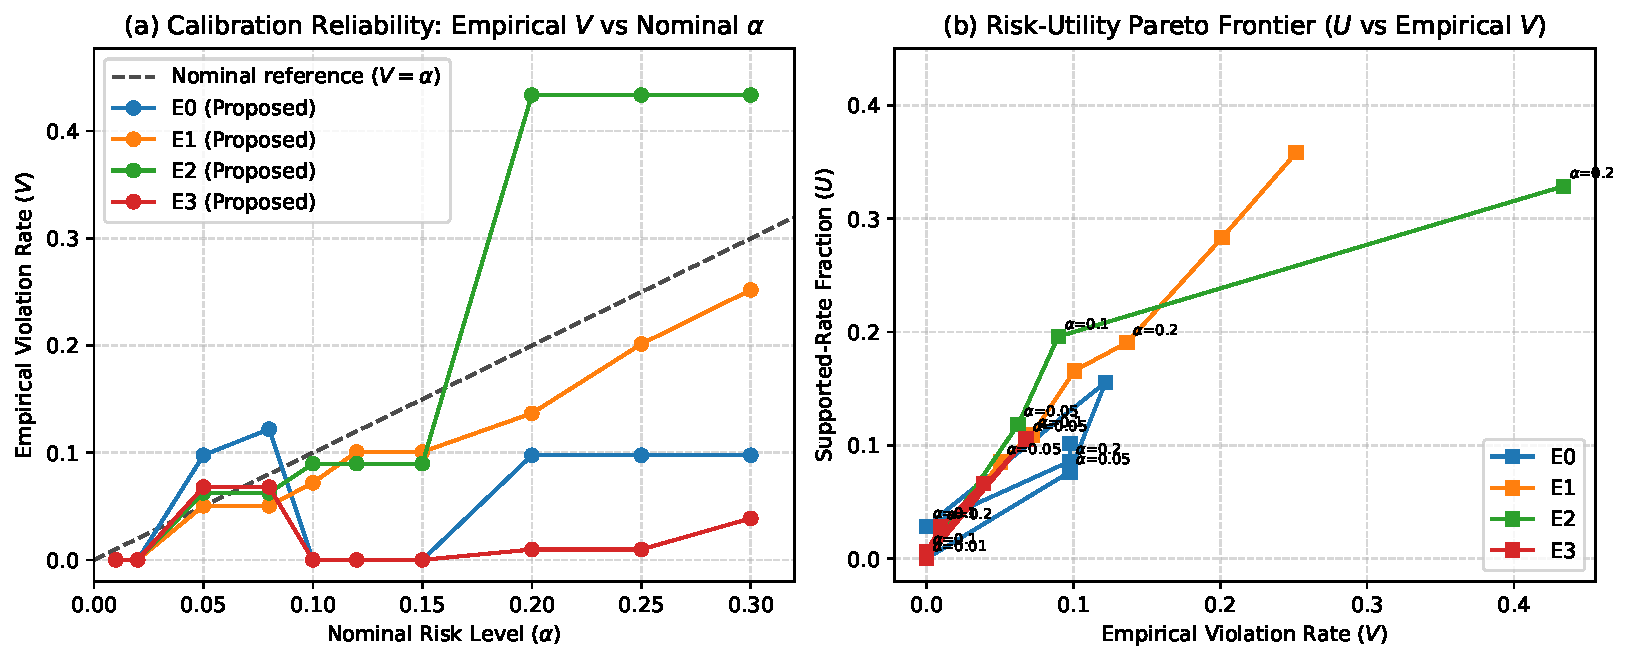
\includegraphics[width=.67\linewidth]{figures/fig4_pareto_frontier.pdf}\caption{Observed violations and supported throughput at the tested nominal levels.}\end{figure}
\begin{figure}[!ht]\centering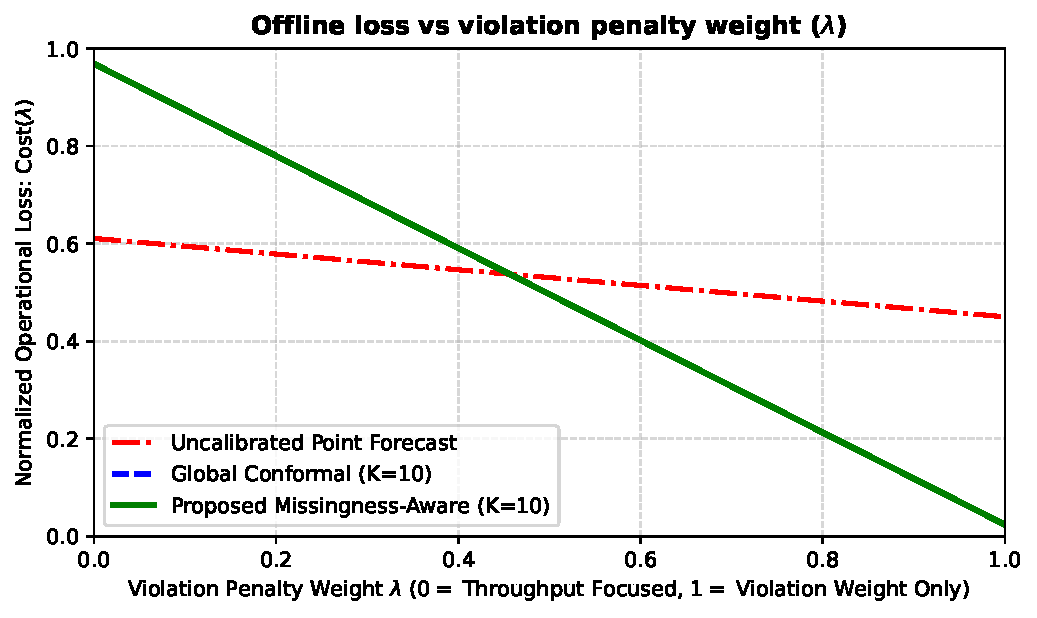
\includegraphics[width=.67\linewidth]{figures/fig5_sla_cost_curve.pdf}\caption{Offline loss under alternative weights on violations and unsupported throughput.}\end{figure}

\begin{table*}[!ht]
\centering\small
\caption{Online feedback and covariate weighting. A uses calibration-pool features and B uses test features. Tight and wide denote weight clipping ranges.}
\begin{tabular}{lrr}
\hline
Protocol & Violation & Supported \\
E0Online & 0.1220 & 0.1762 \\
E1Online & 0.1583 & 0.1653 \\
E2Online & 0.1562 & 0.1775 \\
E3Online & 0.1262 & 0.1447 \\
E1Atight & 0.0072 & 0.0127 \\
E1Awide & 0.0288 & 0.0450 \\
E1Btight & 0.0144 & 0.0063 \\
E1Bwide & 0.0000 & 0.0003 \\
E2Atight & 0.0156 & 0.0304 \\
E2Awide & 0.0156 & 0.0295 \\
E2Btight & 0.0469 & 0.0791 \\
E2Bwide & 0.0664 & 0.1130 \\
E3Atight & 0.0097 & 0.0159 \\
E3Awide & 0.0097 & 0.0083 \\
E3Btight & 0.0000 & 0.0096 \\
E3Bwide & 0.0000 & 0.0085 \\
\hline
\end{tabular}
\end{table*}

\section{Published-baseline and endpoint comparisons}
We reproduced Sirhan's global one-sided forecast on the Irish 5G traces of Raca et al.\ \cite{sirhan2026,raca2020}. Each of 30 splits assigns whole traces to training, calibration and testing. We retained the released features, predictor training and signed-error calibration. For target row $t+1$, persistence uses the downlink measurement at $t-1$, the latest throughput feature available to the tree. A second candidate takes the smaller of that lag and the nonnegative tree estimate before calibration. The Rome experiments informed the candidate choice before its Irish evaluation.

The published frontier chooses among twenty nominal levels using the realized test violations. Table~S6 averages the best supported fractions over feasible splits for each method. At ten percent, 29 splits were feasible for the global rule and all 30 for persistence and the minimum. The paired persistence gain was 3.58 percentage points on the 29 jointly feasible splits. The minimum lost 3.83 points on the corresponding comparison with global.
\begin{table*}[!ht]
\centering\small
\caption{Irish retrospective frontier. Budget and supported throughput are percentages. Gain is persistence minus rerun global in percentage points on jointly feasible splits. Wins counts positive paired gains.}
\begin{tabular}{lrrrrrr}
\hline
Budget & Published & Rerun & Minimum & Persistence & Gain & Wins \\
2 & 33.1 & 33.22 & 32.48 & 34.25 & 1.05 & 13/24 \\
5 & 47.2 & 47.14 & 45.27 & 49.73 & 2.58 & 22/28 \\
10 & 56.9 & 56.98 & 53.30 & 60.54 & 3.58 & 27/29 \\
\hline
\end{tabular}
\end{table*}


At a fixed nominal level of 0.10, all splits contribute. Persistence increased mean supported throughput from 55.60 to 59.44 percent and mean violations from 9.60 to 9.71 percent. Each rule met the ten percent target on 18 of 30 splits. The minimum reduced mean supported throughput to 52.81 percent.
\begin{table*}[!ht]
\centering\small
\caption{Irish fixed nominal ten percent. Mean violation and supported throughput are percentages. Passes counts splits meeting the target out of thirty.}
\begin{tabular}{lrrr}
\hline
Predictor & MeanV & MeanU & Passes \\
Global & 9.60 & 55.60 & 18 \\
Minimum & 9.72 & 52.81 & 17 \\
Persistence & 9.71 & 59.44 & 18 \\
\hline
\end{tabular}
\end{table*}


We kept each fitted forecast and calibration offset fixed and omitted traces only from test scoring. After dropping any one trace from every split in which it appeared, the mean paired gain ranged from 3.53 to 4.64 percentage points. Separately, we averaged each trace's utility difference over its test appearances. Persistence improved 79 of 83 traces, with a median gain of 5.04 points. The five largest download traces contributed 54.4 percent of the sum of measured rates across unique rows. Removing those traces raised the gain to 6.81 points. Removing all 21 download traces left 62 streaming traces and a gain of 10.96 points, alongside a higher violation rate than the tree. These sensitivity estimates reuse overlapping partitions of the same recordings.
\begin{table*}[!ht]
\centering\small
\caption{Irish fixed-setting exclusions from test scoring. Gain is the paired change in supported throughput in percentage points. Wins counts positive splits. Violation rates are percentages.}
\begin{tabular}{lrrrrr}
\hline
Sample & Omitted & Gain & Wins & TreeV & LagV \\
All & 0 & 3.84 & 27 & 9.60 & 9.71 \\
OmitTop5 & 5 & 6.81 & 29 & 5.89 & 7.14 \\
OmitDownloads & 21 & 10.96 & 30 & 2.90 & 4.86 \\
\hline
\end{tabular}
\end{table*}


Table~S9 compares recorded throughput transitions. NearZero counts endpoints at or below 0.001 Mbps. Fall and Rise count changes of at least 10 Mbps from the available lag in the indicated direction. NearZero can overlap Fall. A near-zero measurement does not identify an application stall. In Ireland the lag had a 6.59 Mbps mean absolute error. In the Rome joint shift (E3) it had a 35.44 Mbps error and 40.8 percent of endpoints fell at least 10 Mbps below the lag. On the first ten calibration sessions in E3, persistence supported 51.65 percent with 20.39 percent violations. The tree supported 0.60 percent with zero violations. With the same held-out suffix and eleven disjoint ten-label calibration blocks, persistence met the violation target zero times and the tree eleven times. The higher frequency of large downward changes is consistent with a riskier lag-based lower bound. Forecast horizon, endpoint construction, traffic mix and collection conditions differ together across the two datasets, so this comparison cannot isolate a cause.
\begin{table*}[!ht]
\centering\small
\caption{Lag versus endpoint on unique Irish rows and held-out Rome sessions. MAE is in Mbps. NearZero, Fall and Rise are percentages.}
\begin{tabular}{lrrrrrrr}
\hline
Setting & Pairs & Pearson & Spearman & LagMAE & NearZero & Fall & Rise \\
Ireland & 188545 & 0.77 & 0.67 & 6.59 & 45.0 & 5.8 & 6.3 \\
E0 & 41 & 0.29 & 0.41 & 35.14 & 0.0 & 22.0 & 22.0 \\
E1 & 139 & 0.52 & 0.57 & 32.69 & 7.2 & 37.4 & 14.4 \\
E2 & 256 & 0.70 & 0.61 & 17.57 & 2.0 & 19.1 & 16.0 \\
E3 & 103 & 0.49 & 0.55 & 35.44 & 1.0 & 40.8 & 24.3 \\
\hline
\end{tabular}
\end{table*}

\section{Outcome-independent scheduling and external evaluation}
In the later Rome release, a drop in measured throughput identifies both the start of a segment and the close of its predecessor. An observer who has yet to see that reading cannot identify the same candidate starts. To evaluate a trigger available at forecast time, we used each whole minute of logger operation and required a numeric rate in the preceding minute. Persistence predicts the last available reading in the next minute. We retained the original calendar partitions and calibrated on the first ten labeled opportunities. This changes the endpoint as well as the sample. Of 238 and 171 issued forecasts in E1 and E3, respectively, 211 and 152 had a target in a fully observed window. Missing labels could be informative.

Table~S10 compares the two clock-triggered suffixes with an independent ten-label evaluation on Telenor HSDPA bus measurements released by Riiser et al.\ \cite{riiser2013commute}. We selected all logs on the first route listed by the publisher before measuring forecast performance. At each completed interval we predict the next interval's received bytes per elapsed second, converted to Mbps. Seven chronological dates supply three training dates, two calibration-pool dates and two test dates. The tree uses the last two rates; persistence uses the last rate. Both use the same ten target calibration labels. This evaluates the calibration procedure with a locally fitted predictor. The Irish results in Tables~S6--S8 instead reproduce and extend an existing trace-level protocol. The Norwegian logs lack radio measurements needed to validate the grouped rule.
\begin{table*}[!ht]
\centering\small
\caption{Ten-label calibration for clock-triggered Rome forecasts and Norwegian interval forecasts. Error and offset are in Mbps. Violation and supported fractions are percentages.}
\begin{tabular}{lrrrrrrr}
\hline
Cohort & Model & Scored & Dates & MAE & Offset & Viol & Util \\
E1 & Persistence & 211 & 7 & 44.35 & 114.00 & 8.06 & 8.29 \\
E3 & Persistence & 152 & 7 & 50.72 & 53.90 & 13.82 & 16.00 \\
Norway & Persistence & 1278 & 2 & 0.38 & 1.49 & 0.78 & 26.78 \\
Norway & HistGBM & 1278 & 2 & 0.37 & 1.38 & 1.02 & 30.60 \\
\hline
\end{tabular}
\end{table*}

Fig.~S6 shows how often recalibration clips the commitment to zero at every available prefix length in the primary benchmark. This is the fraction of opportunities on which a lower forecast makes no positive rate commitment.
\begin{figure}[!ht]\centering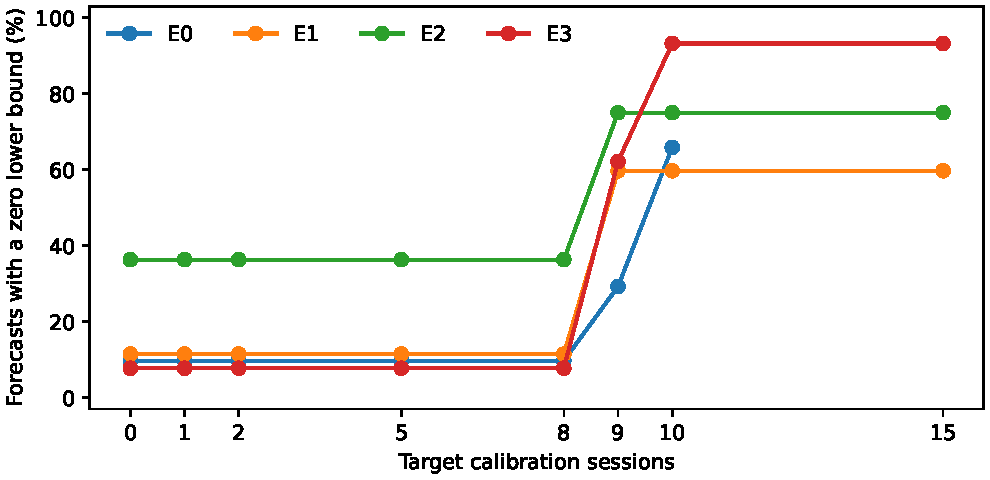
\includegraphics[width=.67\linewidth]{figures/fig6_zero_bounds.pdf}\caption{Fraction of zero global lower bounds by target calibration budget and Rome regime.}\end{figure}

For reset-based persistence in Rome E3, violations and supported throughput were 20.39 and 51.65 percent. With the clock they were 13.82 and 16.00 percent. On the Norwegian route both methods met the empirical violation target on the pooled suffix. Their two test dates provide little information about other days or routes. Neither experiment measures live field application outcomes.
Finally we applied the missingness rule to the Irish measurements in a separate chronological analysis (Table~S11). We used the current availability of numeric primary and NR signal-power fields before any forward filling, the preceding downlink as the point forecast, and the following row as the endpoint. We required strictly ordered lag, issue and target timestamps. The first eleven of 27 collection dates supplied the calibration pool. On the remaining sixteen dates, point MAE was 9.05 Mbps. All first ten calibration rows lacked an NR reading, so both rules gave the same bound on all 108,519 test rows. Violations reached 34.81 percent. Deleting one test date at a time gave 34.03 to 36.68 percent. Even with all 64,265 calibration rows, grouped violations remained 29.86 percent. This failure on a chronological split limits the interpretation of the favorable random-trace results. Split, calibration size and timestamp eligibility differ together.
\begin{table*}[!ht]
\centering\small
\caption{Chronological Irish persistence forecasts on 108519 rows from sixteen suffix dates. Local counts forecasts using a group-specific offset. Performance measures are percentages.}
\begin{tabular}{lrrrrr}
\hline
Labels & Rule & Local & Coverage & Violation & Supported \\
10 & Global & 0 & 65.19 & 34.81 & 71.62 \\
10 & Grouped & 21372 & 65.19 & 34.81 & 71.62 \\
64265 & Global & 0 & 69.50 & 30.50 & 71.31 \\
64265 & Grouped & 108519 & 70.14 & 29.86 & 71.36 \\
\hline
\end{tabular}
\end{table*}

\section{Reliability over all issued commitments}
Let $N$ be the number of issued forecasts, $e$ the observed violations and $m_+$ the positive commitments with unavailable outcomes. Assuming a nonnegative rate exists for each opportunity, the realized violation fraction lies in $[e/N,(e+m_+)/N]$. On missing rows, assigning throughput equal to the commitment attains the lower endpoint; assigning zero attains the upper endpoint. Zero commitments cannot violate. This elementary partial-identification argument follows the logic of worst-case selection bounds \cite{manski1989selection}. It describes a finite ledger. If a forecasted service ceased to exist at trace end, a service-level violation would need its own definition. Sampling uncertainty and conformal expected-risk control \cite{angelopoulos2024risk} answer different questions.

We froze the original tree fitted on 57 earlier Op1 sessions and replayed it alongside persistence. Session features require an explicit clock analogue: lag is the last valid rate in the preceding minute, age is time since that reading, and prior duration is the span between the first and last valid rates in that minute. The six radio fields take their most recent available values strictly before the tick within the same minute. Leaving duration missing gave the same aggregate ten-label tree results. Each policy uses identical ticks, dates, labels and endpoints.

\begin{table*}[!ht]
\centering\footnotesize\setlength{\tabcolsep}{4pt}
\caption{Ten-label Rome clock forecasts. Positive gives measured positive commitments divided by issued positive commitments as counts. Errors counts measured violations. Low and High bound the all-issued violation percentage. U is supported throughput on measured outcomes in percent.}
\begin{tabular}{lllllllll}
\hline
Regime & Predictor & Issued & Scored & Positive & Errors & Low & High & U \\
E1 & Persistence & 238 & 211 & 22/23 & 17 & 7.14 & 7.56 & 8.29 \\
E1 & HistGBM & 238 & 211 & 122/130 & 67 & 28.15 & 31.51 & 7.15 \\
E3 & Persistence & 171 & 152 & 36/37 & 21 & 12.28 & 12.87 & 16.00 \\
E3 & HistGBM & 171 & 152 & 3/3 & 2 & 1.17 & 1.17 & 0.06 \\
\hline
\end{tabular}
\end{table*}

Table~S12 shows that the ten-label tree exceeded the target on E1 even if every unmeasured outcome covered its commitment. On E3 its three positive commitments across 171 opportunities supported just 0.065 percent of measured throughput. Group offsets gave the same bounds at ten labels. Fig.~S7 reports every feasible chronological prefix. For example, at 95 labels the E1 grouped tree violated 21 of 211 measured forecasts (9.95 percent). Six positive commitments lacked outcomes, leaving the all-issued risk between 8.82 and 11.34 percent. This is a retrospective illustration of an unresolved decision.
\begin{figure}[!ht]\centering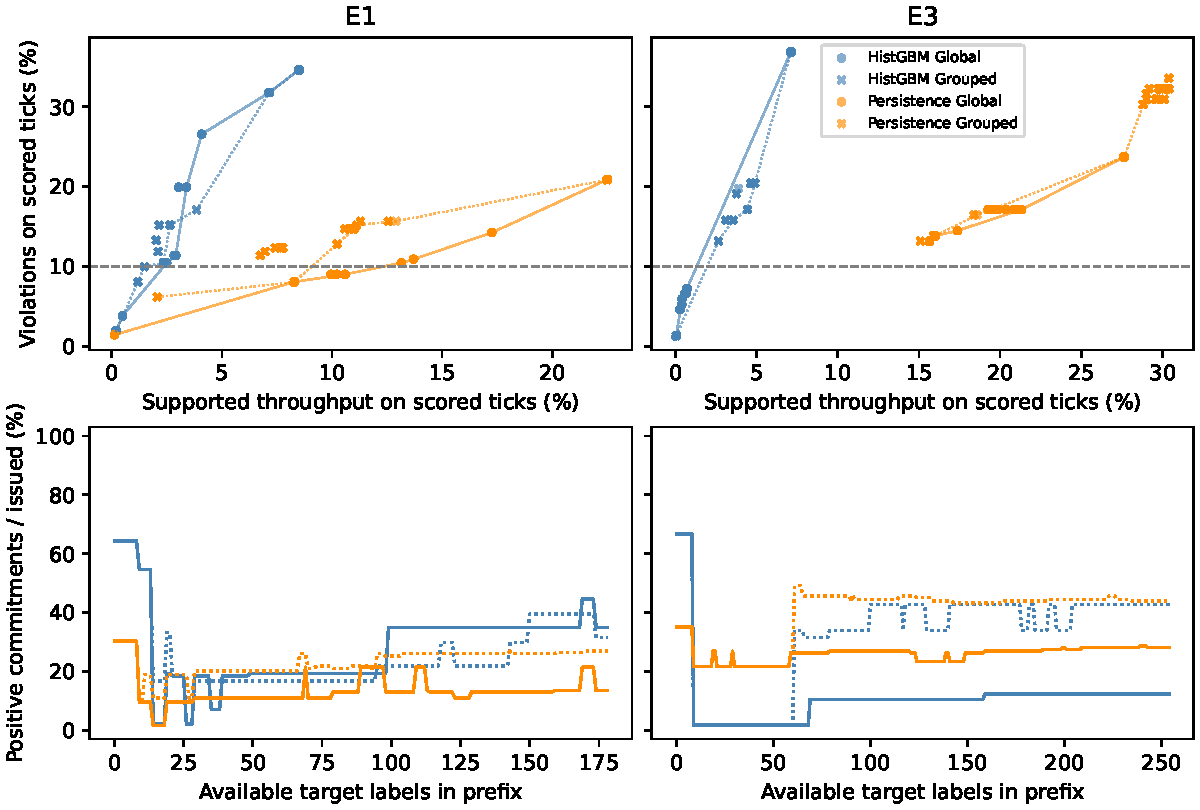
\includegraphics[width=.85\linewidth]{figures/fig7_clock_frontier.pdf}\caption{Rome clock replay at every available prefix size. Each point shows supported throughput and violations on measured outcomes. Lines connect nondominated measured operating points within each policy. The dashed horizontal line is the nominal risk ceiling. The lower panels show the percentage of all issued ticks with a strictly positive commitment at each budget. Solid lines denote global offsets and dotted lines denote grouped offsets.}\end{figure}

At ten labels the E1 tree issued 130 positive commitments. Of the 122 with outcomes, 55 were honored. All three positive E3 commitments occurred on one date and only one was honored. Persistence issued 23 and 37 positive commitments, respectively, of which 22 and 36 were measurable and five and fifteen were honored. For 26 of 27 missing E1 outcomes and all 19 missing E3 outcomes, the recording ended before the forecast horizon. This identifies a limit of observation. The logs cannot establish whether service continued after recording stopped.

We simulated loss of otherwise recorded NR inputs at deployment while holding tick times, measured rates and the ten-label tree offset fixed. On E1, periodic, burst and weak-signal masking reduced supported throughput from 7.15 percent to 5.93, 5.78 and 4.76 percent. Each reduced measured violations as well. Choosing the smaller of each tick's recorded-input and masked-input commitments reduced support to 1.49 percent on E1 and zero on E3. This prediction-based sensitivity envelope describes the implemented tree. It cannot establish the effect of a physical radio outage.

Replacing the first ten tree calibration labels with the latest ten available before each test day reduced E1 measured violations from 31.75 to 4.74 percent and supported throughput from 7.15 to 1.08 percent. On E3, violations increased from 1.32 to 13.16 percent. In a separate same-endpoint Norwegian transfer, the bus-trained tree on three metro test dates supported 5.30 percent with 0.24 percent violations using bus calibration. Ten earlier metro labels changed these to 28.13 and 11.99 percent. A local metro refit and local calibration gave 29.20 and 0.80 percent. Route, dates and predictor must accompany any reported operating point.
An exploratory selection rule maximized validation supported throughput subject to $(e+m_+)/N\leq0.10$. Candidates were zero commitment and both clock predictors with global or grouped offsets at 9, 10, 15 or 20 labels from the first target date. Ties favored smaller budgets, then fixed candidate order. Validation used the remaining pre-test dates (155 measured labels across three dates for E1, 231 across four dates for E3). No offset was refitted. E1 selected nine-label persistence and reproduced the ten-label persistence operating point. E3 selected twenty-label persistence, supporting 19.52 percent of measured throughput with an all-issued violation fraction between 15.20 and 15.79 percent. The fixed ten-label persistence baseline supported 16.00 percent with risk between 12.28 and 12.87 percent. Even with extra validation labels the empirical constraint failed to transfer. The historical test suffix was already known when we designed this analysis.

In an independently collected US drive, we applied ten-label persistence within the publisher's logged AT\&T downlink transfer intervals \cite{nuwinsarchive}. May 13--14, 2023 supplied the calibration pool. Of the two reserved dates, only May 16 contained eligible intervals. Of 36 scheduled ticks, 33 had a preceding rate and all 33 issued forecasts had outcomes. Eight commitments were positive and six violated, giving 18.18 percent all-issued violations and 49.46 percent supported throughput. Three ticks lacked a preceding rate. The time series, device and endpoint differ from Rome. This evaluates the persistence protocol on one informative test date.

\begin{table*}[!ht]
\centering\small
\caption{US Drive 3 with ten earlier labels per carrier. Pos counts issued positive commitments. Fail counts observed violations. Risk bounds and supported throughput are percentages.}
\begin{tabular}{lrrrrrrrr}
\hline
Carrier & Model & Issued & Scored & Pos & Fail & Low & High & U \\
ATT & Persistence & 296 & 294 & 13 & 8 & 2.70 & 2.70 & 7.2872 \\
ATT & Tree & 296 & 294 & 57 & 22 & 7.43 & 7.43 & 2.2524 \\
T-Mobile & Persistence & 294 & 293 & 270 & 201 & 68.37 & 68.37 & 71.5503 \\
T-Mobile & Tree & 294 & 293 & 236 & 123 & 41.84 & 41.84 & 1.2536 \\
Verizon & Persistence & 287 & 283 & 4 & 4 & 1.39 & 1.39 & 0.3845 \\
Verizon & Tree & 287 & 283 & 1 & 0 & 0.00 & 0.00 & 0.0031 \\
\hline
\end{tabular}
\end{table*}

On a second US drive we retained every released carrier and the same ten-label rule. Table~S13 compares persistence and the original Rome-trained tree on identical active-transfer ticks. We aligned six serving-cell signal fields by device timestamp and used only measurements preceding issue. August 5--6 supplied calibration labels. August 7--9 supplied the suffix, with only two scheduled ticks per carrier after midnight on August 9. The three carriers shared the drive. The release lacked the last Verizon raw radio shard; we retained its rates and marked the signals missing.

On AT\&T, 22 of 296 issued tree commitments violated (7.43 percent), including 22 of 57 positive commitments (38.60 percent). T-Mobile had 123 violations among 294 issued and 236 positive commitments. On Verizon the sole positive offer was honored. Masking NR inputs at issue while preserving the full-input tree offset yielded zero positive offers on every carrier. The different carrier operating points and short shared trip limit extrapolation to future deployments.

We also tested feasibility when the 10 percent ceiling applies specifically to positive promises. Selective risk assessment and testing candidate rules motivate this comparison \cite{geifman2017,angelopoulos2021ltt}. On the same pre-test validation dates we scaled each ten-label tree or persistence bound by 0.25, 0.5 or 1. The exploratory service floors required positive offers on at least 10 percent of opportunities and support for at least 5 percent of measured throughput. We counted unresolved positive offers as failures. None of the six candidates met all three empirical criteria on either operator. Requiring a one-sided exact binomial upper limit with a six-way Bonferroni adjustment also yielded no candidate. The quarter-rate E3 tree failed on zero of five positive offers across 252 validation opportunities; its supported fraction was only 0.22 percent. Abstention consequently delivered no service on either suffix. The binomial limit assumes independent offers and supplies no temporal deployment guarantee.

\subsection{Separate trips and client outcomes}
We also replayed the Rome tree on eleven Irish driving-download traces across five held-out dates. The prior all-application calendar cutoff yielded no driving downloads for calibration. Before scoring this cohort, we moved calibration to its first two dates and retained all later dates. Four signal fields map to Rome; both SINR features remain missing. Under the full-minute clock, 334 of 335 ticks had an eligible lag, and 323 had observed outcomes. The tree broke 43 of 155 measurable positive promises, with four more positive promises unresolved. Its all-issued risk was 12.87--14.07 percent and supported throughput 7.74 percent. Persistence broke 31 of 41 positive promises, with all-issued risk 9.28 percent and supported throughput 16.42 percent. On these recordings persistence supported more rate and met the all-issued risk threshold, while failing more often conditional on a positive promise.

To evaluate a client decision, we froze the Norwegian bus-trained lag model and replayed serial two-second video segment requests against measured TCP service on every remaining published route after the original cutoff. Twenty-two recordings on seven routes formed eleven route-date groups across seven calendar dates. Continuity breaks reset the client; each policy used identical blocks. The client selected among five representations from 0.15 to 3 Mbps, starting playback after the first segment and falling back to the lowest representation for smaller commitments. Calibration reduced the stall fraction on all eleven route-dates. Median route-date stall time as a fraction of post-start time fell from 19.12 to 12.93 percent, while median delivered representation fell from 1.01 to 0.24 Mbps. Constant 0.15 Mbps gave 12.30 percent median stalling. These counterfactual playback outcomes assume the measured service is unaffected by request size. They give no direct estimate of user preference or the effect of deploying the client on a live network.

\subsection{Collection-date and client-model sensitivity}
We repeated the fixed-policy summaries with equal weight for each collection date and removed each date in turn. The released ledger provides counts of positive promises, observed failures and unresolved positive outcomes for every date. The Rome E3 tree has positive offers on one of seven test dates; the Verizon tree has them on one of three calendar dates. The final US date contains only a short continuation past midnight. Across five Irish dates, equal-date all-issued risk was 12.43 percent for the tree and 9.43 percent for persistence, with supported throughput 7.09 and 17.31 percent. These are sensitivity descriptions conditional on the archived campaigns. No tick-level confidence interval is used to claim independent replication.

For playback, we varied segment duration over 1, 2 and 4 seconds and a fixed per-request delay over 0, 100 and 300 milliseconds. The representation decision used completed observations at request initiation. All routes on the same calendar date were pooled before comparing policies. On each of seven dates, calibration lowered both stall fraction and delivered bitrate under all nine settings. The median paired stall reduction across dates ranged from 5.50 to 11.81 percentage points; the median bitrate reduction ranged from 0.708 to 0.764 Mbps. This sensitivity supports the direction of the simulated trade-off under those assumptions. Real transport feedback, player buffer limits and user preferences remain outside the model.

\section{Budgeted feedback controller results}
The complete Rome roster contains 254 E1 and 181 E3 scheduled ticks; 238 and 171 respectively have a prior rate. Existing issued-forecast results are unchanged. The US cohorts contain 301, 304 and 292 scheduled ticks, and Ireland 335. A no-lag tick remains in the ledger as ineligible. Each comparison uses the same point predictions and resolved outcomes, so point MAE, RMSE and median error remain constant across policies. Costs distinguish attempted requests from returned labels and residual-buffer updates.

\noindent The retrospective cap-40 controller table appears in the main article.
Fig.~S8 reports the three predefined budgets for the recorded-outcome condition. On E1, MARUR supports 2.02 percent of measured throughput and has 5.46 percent all-issued risk, compared with 1.01 percent support and 5.88--7.14 percent risk for periodic updates. MARUR uses 40 new query attempts, while periodic uses 16; both start with ten successful historical labels. This is an improvement at the same cap with different realized costs. The MARUR tree breaks 13 of 29 positive offers, leaving positive-conditional risk at 44.83 percent. On E3, periodic recalibration supports more throughput with a smaller all-issued upper risk than MARUR. On AT\&T and T-Mobile, increased service under MARUR accompanies greater risk. No uniform superiority is established.

For Ireland MARUR uses 20 new query attempts and supports 1.18 percent, with 12 violations among 155 measured positive offers. Four positive offers are unresolved, so conditional risk lies between 7.55 and 10.06 percent over all 159 positive offers; the measured conditional estimate is 7.74 percent. Periodic supports 2.97 percent using 23 new query attempts, with higher risk. Missing-response suppression also produces mixed effects. On Ireland, conservative residual completion supports 1.17 percent with 3.89 percent all-issued upper risk; dropping unresolved responses supports 3.02 percent with 7.49 percent upper risk. Both incur 20 new attempts, of which only twelve return an outcome. A robust residual bound can trade away service, and it does not by itself control future positive-promise risk.

\begin{figure}[!ht]\centering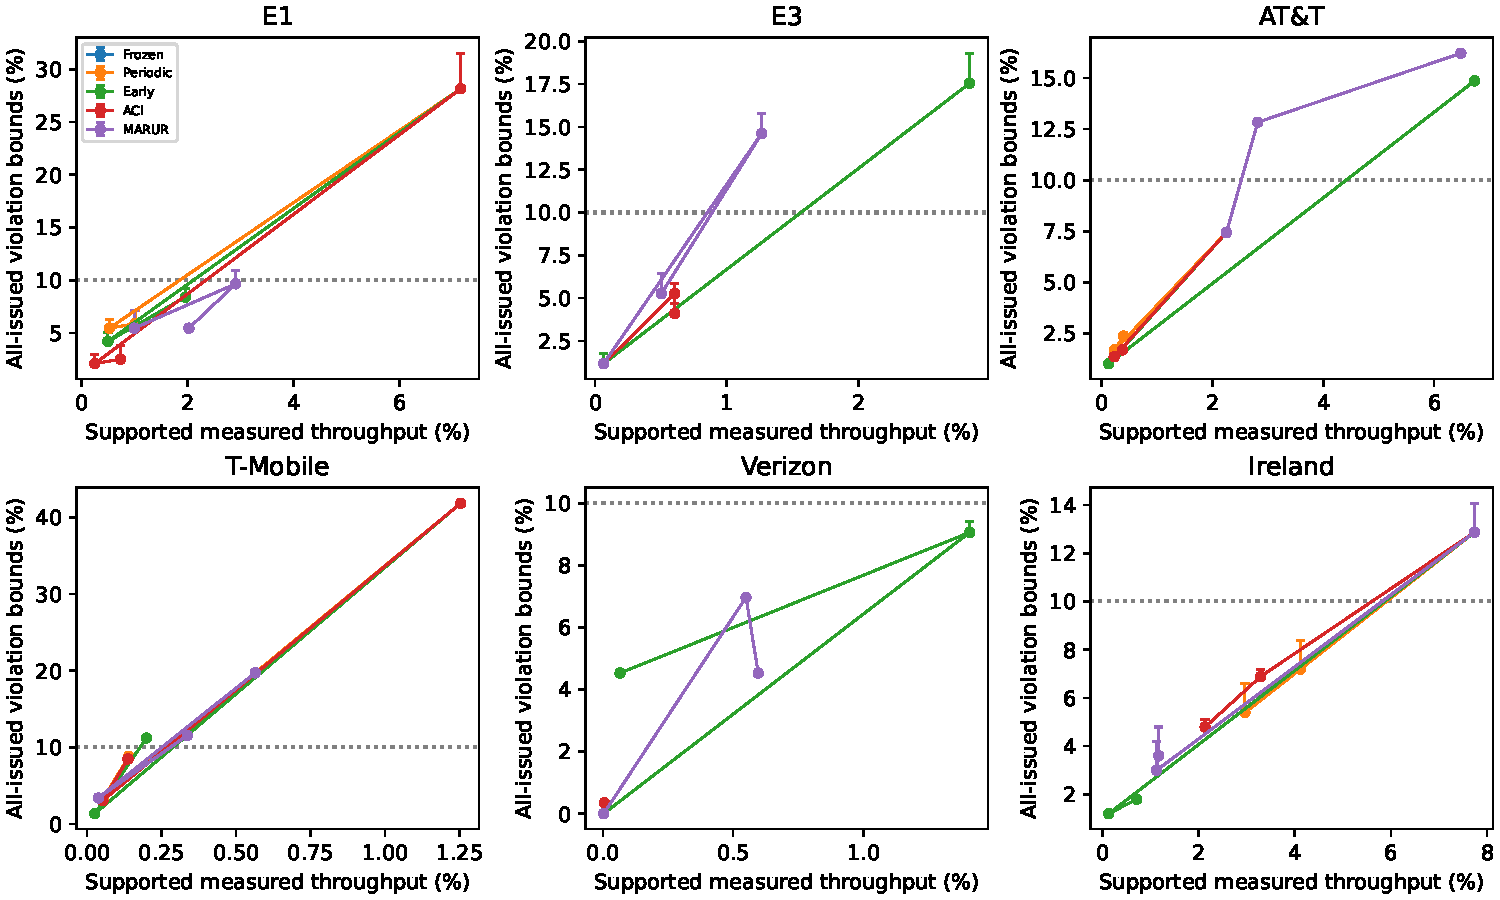
\includegraphics[width=\linewidth]{figures/fig8_marur.pdf}\caption{Frozen-tree controller comparison under new-query caps 0, 10 and 40. Each connected point is a predefined cap, and bars span finite-record all-issued risk bounds. Actual costs differ between schedules. Horizontal axes use observed supported throughput. The nominal ten-percent line is a reference, not a guarantee. All conditional-risk, cost and ablation values are available in the action ledger.}\end{figure}

\subsection{Critical audit at matched realized query cost}
An additional exploratory replay fixes new-query caps at 0, 1, 5, 10, 20 and 40 for Frozen, Periodic, Early, modified ACI and MARUR across all predictors and feedback scenarios (576 original runs, 720 full-suffix replays, and 384 exact-cost pairs; complete cap-40 six-cohort breakdown in Table~S14). Frozen spends zero and is therefore not a positive-cost comparator. No interpolation, shortened suffix or test-selected deployment policy is used.

\begin{table*}[!ht]
\centering\small
\caption{Retrospective six-cohort controllers at new-query cap 40 under frozen HistGBM and recorded feedback (with ten initial successful labels).}
\begin{tabular}{lrrrrrr}
\hline
Cohort & Policy & Queries & Offers & PosLow & PosHigh & U \\
E1 & Frozen & 0 & 130 & 51.54 & 57.69 & 7.154 \\
E1 & Periodic & 16 & 33 & 42.42 & 51.52 & 1.008 \\
E1 & MARUR & 40 & 29 & 44.83 & 44.83 & 2.025 \\
E3 & Frozen & 0 & 3 & 66.67 & 66.67 & 0.065 \\
E3 & Periodic & 12 & 16 & 43.75 & 50.00 & 0.605 \\
E3 & MARUR & 29 & 20 & 45.00 & 55.00 & 0.504 \\
ATT & Frozen & 0 & 57 & 38.60 & 38.60 & 2.252 \\
ATT & Periodic & 20 & 30 & 23.33 & 23.33 & 0.402 \\
ATT & MARUR & 40 & 111 & 43.24 & 43.24 & 6.481 \\
T-Mobile & Frozen & 0 & 236 & 52.12 & 52.12 & 1.254 \\
T-Mobile & Periodic & 20 & 47 & 55.32 & 55.32 & 0.141 \\
T-Mobile & MARUR & 40 & 52 & 65.38 & 65.38 & 0.337 \\
Verizon & Frozen & 0 & 1 & 0.00 & 0.00 & 0.003 \\
Verizon & Periodic & 20 & 5 & 20.00 & 20.00 & 0.006 \\
Verizon & MARUR & 40 & 21 & 61.90 & 61.90 & 0.597 \\
Ireland & Frozen & 0 & 159 & 27.04 & 29.56 & 7.740 \\
Ireland & Periodic & 23 & 159 & 11.32 & 13.84 & 2.966 \\
Ireland & MARUR & 20 & 159 & 7.55 & 10.06 & 1.175 \\
\hline
\end{tabular}
\end{table*}


At ten new queries with the frozen tree, MARUR's E1 support is 2.907 percent versus Periodic's 0.523 percent, but its all-issued upper risk is 10.924 versus 6.303 percent. On Ireland both make 159 positive offers: MARUR has fourteen fewer observed failures on those same offers while reducing support from 4.117 to 1.129 percent. This is smaller commitment size rather than increased abstention. On Verizon, MARUR removes ten of Early's offers and six failures, without improving failures on shared offers. Complete costs, conditional risks, offer frequencies and date counts for every configuration are in the matched-cost supplement. These examples do not establish uniform superiority.

The audit also clarifies that failed responses reset the query cooldown even when their score is discarded. Removing pattern dependence jointly removes triggering, gating and grouping, so it is not an isolated gate ablation. The synthetic missing-feedback mask applies to eligible positions divisible by five; periodic positions 1, 16, 31 and so on avoid it. It is therefore position-based censoring, not a uniform twenty-percent loss of requested labels.

\section{Limitations, comparator taxonomy, and extended exploratory checks}
These archives were inspected before the controller and cost audit were designed. The 384 exact-cost contrasts are descriptive comparisons of shared observations, not independent trials or confirmatory tests. Missing-outcome intervals are finite-record partial-identification bounds, not sampling confidence intervals. A low all-issued risk can result from abstention; positive-conditional risk and useful service must be reported jointly. The modified ACI comparator, bundled pattern ablation and position-based feedback suppression limit method-specific conclusions. All evidence is retrospective from public archives and no live field validation was performed; simultaneous carriers do not increase independent campaign-dates, and simulated playback does not establish causal live QoE.

\subsection{Comparator taxonomy, PACER protocol details, and extended exploratory sweeps}
To avoid post-hoc tuning on the held-out public archives (Rome Capacity Op1, Rome Capacity Op2, Oslo Commute, Ireland Static; accessed prior to evaluation), all PACER parameters ($\alpha=0.10$, $\gamma=0.05$, $a_{\text{veto}}=0.15$, $\kappa_{\text{ext}}=2.0$, $W_{\text{obs}}=20$, seeds 42, 123, and 2026, caps 0, 10, and 40) were frozen and SHA-256 locked before scoring those archives, following retrospective analysis of MARUR failure modes. Table~S15 summarizes the operational taxonomy comparing MARUR and PACER across regimes, Table~S16 reports the complete 18-row pooling-rule sensitivity matrix across HeldOut, Retrospective, and AllCohorts scopes, Table~S17 reports the complete 11-row Leave-One-Cohort-Out check across all 10 cohorts (42 total clusters), Table~S18 reports the exploratory campaign-level dependence sensitivity over the 3 retrospective and 3 held-out geographic campaigns (contrasting naive equal-cluster $\pm 50\%$ TOST $p$ against Donner campaign-adjusted $\pm 50\%$ and $\pm 25\%$ relative TOST $p$-values, adjusted $\pm 2$~pp $p$, effective date counts $G_{\text{eff}}$, and two-stage hierarchical bootstrap 90\% equal-cluster relative intervals), and Table~S19 reports both per-campaign risk/utility medians and the 6-campaign Leave-One-Campaign-Out (LOCampO) robustness check removing all co-located carrier links of each field campaign together. Across all 120 seed-sensitivity evaluations (QueryCensor20 and Persistence included), weighted selective excess lies within $B_1(K) \approx 6.8/K$ on 40/40 cells, though as established in the main manuscript this bound holds trivially on 36/40 cells whenever $B_1(K) \ge (1-\alpha)A$ (19/20 cells at $C_{\text{new}}=10$ and 17/20 at $C_{\text{new}}=40$). Under Persistence across all 42 pooled clusters, PACER's conservative abstention lowers utility $U$ by $-18.89$ percentage points at cap 10 (bootstrap $-31.02$ to $-3.25$) and $-29.95$ percentage points at cap 40 (bootstrap $-37.26$ to $-16.39$) relative to Frozen. For the exploratory controlled-freshness 1,848-configuration grid across recorded and masked stresses, completed versus observed clocks yield 6 matched utility gains without higher conditional upper risk, 7 losses without lower risk, 8 trade-offs or risk-only changes, 129 unchanged cases, and 18 unmatched-cost cases; across the 792 configurations of the targeted baseline grid, pattern versus pooled quantiles give identical utility and conditional risk in all 72 paired configurations with the gate fixed, removing only the gate produces 16 utility gains without higher upper risk, 10 trade-offs/risk-only changes, and 46 unchanged cases, DecayingOGD versus Periodic yields 9 utility gains without higher upper risk, 18 losses without lower risk, and 45 trade-offs or risk-only changes, and reconstructed Verizon window-20 scores tie a conservative missing-response penalty at the quantile on 159 of 287 eligible ticks. Complete ledgers (including the extended 1,800-run retrospective/held-out window and $\alpha$ sweep and 480-run source-only predictor sweep for both MARUR and PACER, as well as the Oslo Commute pre-2010 bus quantile regressor check) reside in \texttt{results/pacer} and \texttt{results/exploratory/sensitivity}.

\begin{table*}[!ht]
\centering\footnotesize\setlength{\tabcolsep}{3.5pt}
\caption{Operational comparator taxonomy across regimes, assumptions, and primary failure modes (rates and differences in percent / percentage points).}
\begin{tabular}{lllll}
\hline
Regime & Method & Property & ObservedMetric & PrimaryFailure \\
Static high offer (A at least 0.50) & PACER & T1 O(1/K) & 5.12-6.98 PosHi IrelandSt & Needs horizon length T \\
Budget-starved multi-day (C=10) & PACER & T2 Wmax blk & -23.41pp OfferWtd vs Per & Driven by Oslo offers \\
Short rapid shift (C=40, T 300) & MARUR & Heuristic W=10 & Forgets init faster on Op1 & Day-1 churn; miss freeze \\
Stationary / Retro C=40 & Periodic & Fixed cadence & 35.67 vs PAC 47.81 PosHi & Day-1 blind when P x C low \\
Low A or uncalibrated Persist & Halt/Refuse & Fail safe & Avoids -29.95pp U drop & No SLA rate valid \\
\hline
\end{tabular}
\end{table*}


\begin{table*}[!ht]
\centering\footnotesize\setlength{\tabcolsep}{3.5pt}
\caption{Complete 18-row pooling-rule sensitivity for PACER minus Periodic contrasts across HeldOut, Retrospective, and AllCohorts (HistGBM, recorded, percentage points).}
\begin{tabular}{lllllll}
\hline
Scope & Cap & WeightRule & Units & dPosHi & Boot95 & dU \\
HeldOut & 10 & OfferWtd & 26 & -23.41 & -37.04 to -5.91 & +0.47 \\
HeldOut & 10 & EqualUnit & 22/26 & +0.37 & paired valid & -3.29 \\
HeldOut & 10 & EqualCohort & 4 coh & -4.88 & unweighted & -2.91 \\
HeldOut & 40 & OfferWtd & 26 & -0.83 & -16.13 to +11.46 & +0.51 \\
HeldOut & 40 & EqualUnit & 12/26 & +2.79 & paired valid & +0.01 \\
HeldOut & 40 & EqualCohort & 4 coh & +5.08 & unweighted & +0.56 \\
Retrospective & 10 & OfferWtd & 16 & +8.83 & -2.16 to +13.99 & +0.11 \\
Retrospective & 10 & EqualUnit & 10/16 & -4.36 & paired valid & -0.10 \\
Retrospective & 10 & EqualCohort & 6 coh & +6.02 & unweighted & +0.13 \\
Retrospective & 40 & OfferWtd & 16 & +16.26 & +4.68 to +24.93 & +0.19 \\
Retrospective & 40 & EqualUnit & 9/16 & -5.93 & paired valid & +0.05 \\
Retrospective & 40 & EqualCohort & 6 coh & +12.15 & unweighted & +0.08 \\
AllCohorts & 10 & OfferWtd & 42 & -14.37 & -26.80 to +0.85 & +0.25 \\
AllCohorts & 10 & EqualUnit & 32/42 & -1.11 & paired valid & -2.07 \\
AllCohorts & 10 & EqualCohort & 10 coh & +1.66 & unweighted & -1.09 \\
AllCohorts & 40 & OfferWtd & 42 & +3.29 & -7.49 to +12.49 & +0.31 \\
AllCohorts & 40 & EqualUnit & 21/42 & -0.94 & paired valid & +0.02 \\
AllCohorts & 40 & EqualCohort & 10 coh & +9.32 & unweighted & +0.27 \\
\hline
\end{tabular}
\end{table*}


\begin{table*}[!ht]
\centering\footnotesize\setlength{\tabcolsep}{3.5pt}
\caption{Leave-one-cohort-out check across all 10 cohorts (42 total clusters, HistGBM, recorded feedback). Mobile risk range excludes static Ireland; U is median supported throughput.}
\begin{tabular}{llllllll}
\hline
Dropped & G & MobRhiRng & MobRhiMed & UMed & EqdU MAR10 & EqdU PAC10 & EqdU PAC40 \\
None & 42 & 8.8-68.2 & 47.6 & 1.01 & -2.11 & -2.07 & +0.02 \\
ATT & 42 & 8.8-68.2 & 48.5 & 1.01 & -2.13 & -2.08 & +0.02 \\
E1 & 41 & 8.8-66.7 & 47.3 & 0.90 & -2.27 & -2.25 & +0.03 \\
E3 & 41 & 8.8-68.2 & 47.1 & 1.15 & -2.16 & -2.07 & -0.00 \\
Ireland & 37 & 16.2-68.2 & 49.3 & 0.67 & -2.07 & -2.24 & -0.05 \\
Ireland Static & 38 & 8.8-68.2 & 47.6 & 1.15 & -2.35 & -2.34 & -0.46 \\
Oslo Commute & 35 & 8.8-68.2 & 49.1 & 0.67 & +0.36 & +0.12 & -0.04 \\
Rome Capacity Op1 & 42 & 8.8-68.2 & 47.9 & 0.76 & -1.93 & -1.83 & +0.26 \\
Rome Capacity Op2 & 42 & 8.8-68.2 & 47.4 & 0.76 & -2.29 & -2.38 & -0.55 \\
T-Mobile & 42 & 8.8-68.2 & 47.3 & 1.17 & -2.06 & -2.06 & +0.04 \\
Verizon & 42 & 8.8-68.2 & 47.5 & 1.17 & -2.12 & -2.07 & +0.02 \\
\hline
\end{tabular}
\end{table*}


\begin{table*}[!ht]
\centering\footnotesize\setlength{\tabcolsep}{2.2pt}
\caption{Exploratory campaign-level dependence sensitivity across physical geographic campaigns (Camp=3 Retrospective, 3 HeldOut, 6 AllCohorts; HistGBM, recorded). Compares naive equal-cluster +-50 percent relative TOST p (Naive50) with Donner-adjusted relative TOST p (Adj50, Adj25), adjusted +-2 pp p (Adjp2), effective date count (Geff), adjusted MDE80 (pp), and two-stage hierarchical bootstrap 90 percent equal-cluster relative intervals (percent).}
\begin{tabular}{llrrrrrrrrrrrr}
\hline
Scope & Cand & Cap & G & Camp & ICC & DEFF & Geff & Naive50 & Adj50 & Adj25 & Adjp2 & AdjMDE & HierBoot90Rel \\
Retro & MAR & 10 & 16 & 3 & 0.62 & 4.16 & 3.84 & 0.1228 & 0.2988 & 0.4084 & 0.0971 & 4.93 & -79.5 to +512.0 \\
Retro & PAC & 10 & 16 & 3 & 0.02 & 1.08 & 14.77 & 0.0430 & 0.0498 & 0.2332 & 0.0001 & 1.13 & -45.3 to +268.9 \\
Retro & MAR & 40 & 16 & 3 & 0.14 & 1.72 & 9.28 & 0.1535 & 0.2215 & 0.3889 & 0.0099 & 2.05 & -65.6 to +401.6 \\
Retro & PAC & 40 & 16 & 3 & 0.00 & 1.00 & 16.00 & 0.0426 & 0.0426 & 0.2036 & 0.0000 & 1.00 & -69.8 to +79.0 \\
HeldOut & PAC & 10 & 26 & 3 & 0.81 & 9.24 & 2.81 & 0.5369 & 0.5108 & 0.6370 & 0.6052 & 26.06 & -65.7 to +76.6 \\
HeldOut & MAR & 10 & 26 & 3 & 0.82 & 9.36 & 2.78 & 0.5497 & 0.5144 & 0.6255 & 0.5973 & 30.33 & -71.7 to +111.8 \\
HeldOut & PAC & 40 & 26 & 3 & 0.28 & 3.87 & 6.73 & 0.0071 & 0.1153 & 0.2653 & 0.1388 & 5.64 & -64.0 to +115.0 \\
HeldOut & MAR & 40 & 26 & 3 & 0.41 & 5.15 & 5.05 & 0.0291 & 0.2153 & 0.4911 & 0.2623 & 4.92 & -42.6 to +5.1 \\
AllCoh & PAC & 10 & 42 & 6 & 0.76 & 7.23 & 5.81 & 0.4237 & 0.4727 & 0.6461 & 0.5119 & 8.49 & -60.9 to +39.3 \\
AllCoh & PAC & 40 & 42 & 6 & 0.17 & 2.40 & 17.48 & 0.0021 & 0.0341 & 0.1754 & 0.0145 & 2.46 & -50.6 to +93.9 \\
\hline
\end{tabular}
\end{table*}


\begin{table*}[!ht]
\centering\footnotesize\setlength{\tabcolsep}{3.5pt}
\caption{Leave-one-campaign-out (LOCampO) robustness and per-campaign medians across all 6 physical field campaigns (HistGBM, recorded; percentages and percentage points). None denotes full 6-campaign pool; CampRhiMed and CampUMed report the omitted campaign median across cap in {10, 40}.}
\begin{tabular}{lllllllll}
\hline
DroppedCamp & RemC & G & CampRhiMed & CampUMed & RemMobRhiMed & RemUMed & EqdU PAC10 & EqdU PAC40 \\
None & 6 & 42 & 47.1 & 1.01 & 47.6 & 1.01 & -2.07 & +0.02 \\
Ireland Drive & 5 & 37 & 15.7 & 2.93 & 49.3 & 0.67 & -2.24 & -0.05 \\
Ireland Static & 5 & 38 & 6.0 & 0.35 & 47.6 & 1.15 & -2.34 & -0.46 \\
Oslo Commute & 5 & 35 & 23.1 & 11.37 & 49.1 & 0.67 & +0.12 & -0.04 \\
Rome 2023 & 5 & 34 & 54.2 & 0.61 & 45.8 & 1.15 & -2.63 & +0.11 \\
Rome Capacity & 5 & 27 & 47.5 & 1.35 & 47.9 & 0.61 & -3.38 & +0.81 \\
US Drive3 & 5 & 39 & 47.9 & 0.35 & 47.5 & 1.28 & -2.25 & +0.01 \\
\hline
\end{tabular}
\end{table*}


\section{Conclusion}
The budgeted controller demonstrates why attempted measurements, returned labels and useful positive commitments must be counted separately. Its recorded improvements do not persist uniformly across cohorts; exact-cost contrasts are separately reported in the critical audit supplement. MARUR therefore serves as an empirical risk-aware framework with a reproducible causal ledger, while stronger adaptive-method and deployment claims require additional evidence.
The same frozen tree failed the ten-percent target on one clock-triggered suffix and supported almost no throughput on the other. Missing labels can change whether the target is decidable; their impact depends on how often the forecaster actually commits a positive rate. Moving the calibration window or conditioning on radio availability did not produce a consistent improvement. More independent dates and logged test-start events are needed to assess future deployments.
\section*{Acknowledgment}
OpenAI Codex assisted with code development, experimental checks and drafting and revising the manuscript.
\bibliographystyle{IEEEtran}
\bibliography{references}
\end{document}
